\documentclass[12pt]{article}                         
\pagestyle{plain}

\usepackage{amsmath}     % Enhanced math environments (e.g., align).
\usepackage{amsfonts}    % Math fonts (e.g., \mathfrak{}).
\usepackage{amstext}     % Text inside math mode (e.g., \text{where}).
\usepackage{amssymb}     % Extra math symbols (e.g., \mathbb{R}).
\usepackage{array}       % Advanced table/array column definitions.
\usepackage{circledtext} % Puts text inside a circle (e.g., \circledtext{A}).
\usepackage{comment}     % Include/exclude blocks of text.
\usepackage{enumerate}   % Customize itemized/numbered lists.
\usepackage{graphicx}    % Include images/graphics (\includegraphics).
\usepackage{latexsym}    % Access to basic LaTeX symbols.
\usepackage{multicol}    % Allows text columns on a page.
\usepackage{pgfplots}    % Create scientific plots from data (based on TikZ).
\usepackage{tabularx}    % Tables that stretch to page width.
\usepackage{tasks}       % Create multi-column lists.
\usepackage{textcomp}    % Provides many text symbols (e.g., \textcelsius).
\usepackage{tikz}        % Create vector graphics and diagrams.
\usepackage{xcolor}      % Define and use colors.
\usepackage{fancyhdr}
\usepackage{tcolorbox}
\usepackage{enumitem}
\pgfplotsset{compat=1.18}

\usepackage[
  letterpaper,
  left=0.8in,
  right=0.8in,
  textheight=9.5in,
  bmargin=0.5in  % Adjust this value to push the footer down
]{geometry}
\pagestyle{fancy}
\fancyhf{} % Clear all header and footer fields
\fancyhead[L]{Your Name:} % Left header with name
\fancyhead[R]{December 2nd 2025} % Right header with date
\renewcommand{\headrulewidth}{0.4pt} % Horizontal line below the header

\begin{document}

% Main title
\begin{center}
    \Large \textbf{Math 115E Activity 21} \\
    \vspace{0.2cm}
    \normalsize Chapter 7: Polynomials \\
    \normalsize Multiplicities
\end{center}
\vspace{-0.5cm}
\subsection*{Multiplicities of Polynomials}

\begin{tcolorbox}[
    width=\linewidth,
    colframe=black,         % Border color
    colback=white,          % Background color
    boxrule=0.5pt,          % Border thickness
    left=1mm, right=1.1mm,  % Horizontal padding
    top=1mm, bottom=1mm,    % Vertical padding
    arc=2mm                 % Corner radius
]
\textbf{Reminder:} 
\textit{Given a function $f(x)$ and knowing that points are of the form $(x,y)$, 
\begin{itemize} 
    \item The x-intercepts are when $y=0$, the coordinate points of the form $(x,0)$ on the function
    \item The y-intercept is when $x=0$, the coordinate points of the form $(0,f(0))$ on the function
\end{itemize}}
\end{tcolorbox}
\begin{tcolorbox}[
    width=\linewidth,
    colframe=black,         % Border color
    colback=white,          % Background color
    boxrule=0.5pt,          % Border thickness
    left=1mm, right=1.1mm,    % Horizontal padding
    top=1mm, bottom=1mm,    % Vertical padding
    arc=2mm                 % Corner radius
]
\textbf{Definition:} 
\textit{Given a polynomial $f(x)$, the number of times a given term $(x-c)$ 
appears in the factored form of $f(x)$ is called the \textbf{multiplicity}}
\end{tcolorbox}
\noindent\\
Example: If we have the polynomial: $g(x) = (x-1)(x-2)^4(x+3)^3(x+4)^2$
\begin{itemize}
    \item Then we can say the following solutions are $x= 1, x= 2,x= -3,x= -4$ 
    \item Now, notice that: $x=\hphantom{-}1$ has a multiplicity of 1, and $x=\hphantom{-}2$ has a multiplity of 4 \\
    \hspace*{90pt} $x=-3$ has a multiplicity of 3, and $x=-4$ has a multiplity of 2
    \item The only y-intercepts is at $f(0)=(0-1)(0-2)^4(0+3)^3(0+4)^2=(-1)(-2)^4(3)^3(4)^2=-6912$
    \item The multiple x-intercepts are solutions of $0=f(x)$ which are $(1,0), (2,0),(-3,0),(-4,0)$
\end{itemize}
\noindent\\
For the following problems, x-intercepts, their multiplicities, and the y-intercepts
\begin{enumerate}
    \item[\#1] $f(x) = (x-2)^3(x-1)$
    \\\\\\
    \item[\#2] $f(x) = (x+1)^2(x-1)$
    \\\\\\
    \item[\#3] $f(x) = (x^2-4)(x+3)^3$
    \\\\\\
    \item[\#4] $f(x) = (x-1)^4(x^2+3)(x+2)^2$
    \\\\\\
    \item[\#5] $f(x) = x(x^2-2)(x-3)^3(x+4)^2$
\end{enumerate}

\subsection*{Graphing Multiplicities}
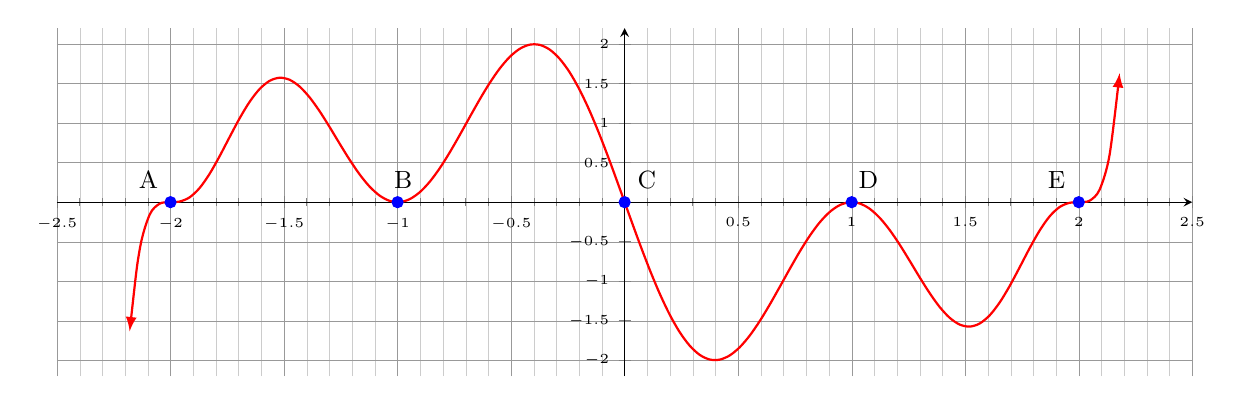
\begin{tikzpicture}
\begin{axis}[
    % Set the overall dimensions of the plot area
    height=6cm, 
    width=16cm,  
    % Set the domain and range for the axes
    xmin=-2.5, xmax=2.5,
    ymin=-2.2, ymax=2.2,
    % Manually set the tick marks
    xtick={-2.5,-2,-1.5,-1,-0.5,0,0.5,1,1.5,2,2.5},
    ytick={-2.5,-2,-1.5,-1,-0.5,0.5,1,1.5,2,2.5},
    % Add 5 minor lines between each major tick on both axes
    minor x tick num=4,
    minor y tick num=4,
    % This command draws both major and minor grid lines
    grid=both,
    major grid style={line width=.1pt,draw=gray!80},
    minor grid style={line width=.1pt,draw=gray!40},
    % Axis and label styling
    axis lines=middle,
    tick label style={font=\tiny},
    xlabel style={at={(current axis.right of origin)}, anchor=west},
    ylabel style={at={(current axis.above origin)}, anchor=south},
    axis line style={-stealth}
]

\addplot[domain=-2.18:2.18, smooth, samples=100, thick, red,latex-latex] {(1/8)*x*(x+1)^2*(x-1)^2*(x-2)^3*(x+2)^3};
\draw[fill=blue, draw=blue] (-2, 0)   circle (2pt) 
    node[xshift=-8pt, yshift=8pt, font=\small] {A};

\draw[fill=blue, draw=blue] (-1, 0)   circle (2pt) 
    node[xshift=2pt, yshift=8pt, font=\small] {B};

\draw[fill=blue, draw=blue] (0, 0)   circle (2pt) 
    node[xshift=8pt, yshift=8pt, font=\small] {C};

\draw[fill=blue, draw=blue] (1, 0)   circle (2pt) 
    node[xshift=6pt, yshift=8pt, font=\small] {D};

\draw[fill=blue, draw=blue] (2, 0)   circle (2pt) 
    node[xshift=-8pt, yshift=8pt, font=\small] {E};

\end{axis}
\end{tikzpicture}\\
\noindent
We have 5 intercepts for the following function as described on the above graph \\
assume their multiplities are the smallest that they can be.\\\\
\noindent
Let's find the multiplities of each intercept and their value
\begin{itemize}
    \item Intercept A:\\
    \item Intercept B:\\
    \item Intercept C:\\
    \item Intercept D:\\
    \item Intercept E:\\
\end{itemize}
What do we think the smallest degree of the polynomial will be?
\\\\
\noindent
Sketch graph of the following function: $f(x)=\frac{1}{40}x(x+1)(x-2)^2(x-3)^2$\\
Use the end behavior, x intercepts, and the multiplicities of the following function:\\
\hspace{-1.2cm}
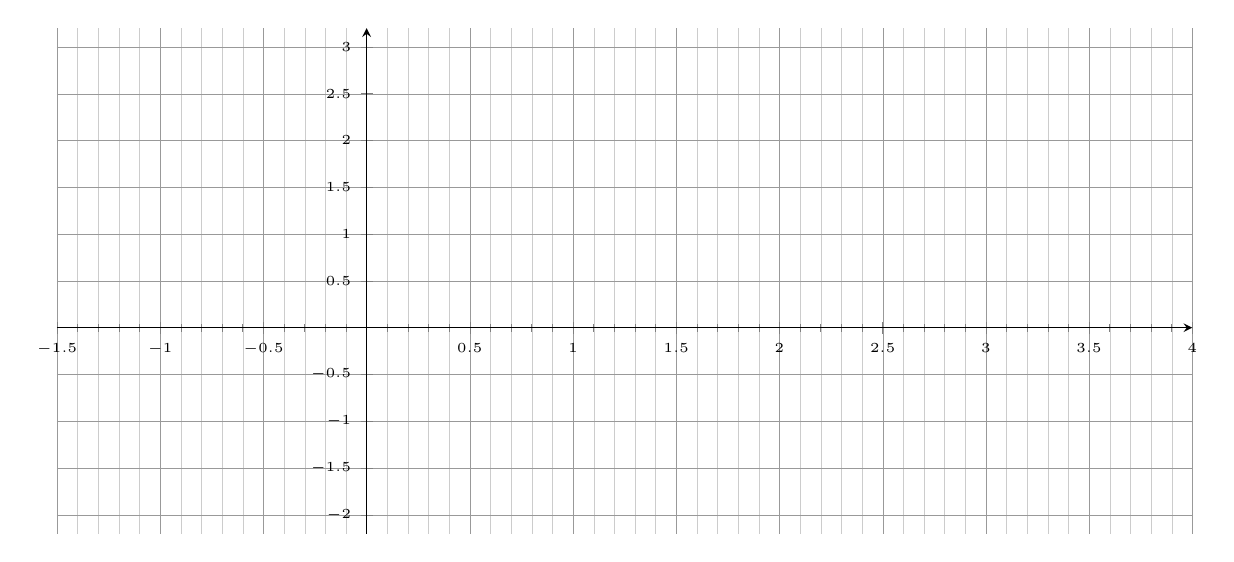
\begin{tikzpicture}
\begin{axis}[
    % Set the overall dimensions of the plot area
    height=8cm, 
    width=16cm,  
    % Set the domain and range for the axes
    xmin=-1.5, xmax=4,
    ymin=-2.2, ymax=3.2,
    % Manually set the tick marks
    xtick={-1.5,-1,-0.5,0,0.5,1,1.5,2,2.5,3,3.5,4},
    ytick={-2,-1.5,-1,-0.5,0.5,1,1.5,2,2.5,3},
    % Add 5 minor lines between each major tick on both axes
    minor x tick num=4,
    minor y tick num=4,
    % This command draws both major and minor grid lines
    grid=both,
    major grid style={line width=.1pt,draw=gray!80},
    minor grid style={line width=.1pt,draw=gray!40},
    % Axis and label styling
    axis lines=middle,
    tick label style={font=\tiny},
    xlabel style={at={(current axis.right of origin)}, anchor=west},
    ylabel style={at={(current axis.above origin)}, anchor=south},
    axis line style={-stealth}
]

%\addplot[domain=-1.5:3.8, smooth, samples=100, thick, red,latex-latex] {(1/10)*x*((x+1))*((x-2)^2)*((x-3)^2)};


%had a small typo for the above function, plus the shape doesnt look the greatest but its okay
% next time show degree and multiplicities and if there are some values missing
\end{axis}
\end{tikzpicture}
\end{document}